% Root document for the thesis draft chapters.
% Self-contained under /home/gio/tese (figures in ./figuras/eda/).
% Build:  latexmk -pdf tese.tex     (or: pdflatex tese.tex  x2)
\documentclass[12pt,a4paper]{book}

\usepackage[T1]{fontenc}
\usepackage[utf8]{inputenc}
\usepackage[english]{babel}
\usepackage{amsmath}
\usepackage{amssymb}
\usepackage{siunitx}
\sisetup{round-mode=none}
\DeclareSIUnit{\flop}{FLOP}  % used by the aiconfigurator chapter (TFLOP/s)
\usepackage{booktabs}
\usepackage{graphicx}
\usepackage{microtype}

\title{Thesis Draft Chapters --- Workspace Preview Build}
\author{Giovanni Oliveira}
\date{\today}

\begin{document}
\maketitle
\tableofcontents

%!TeX root=../tese.tex
\chapter{Calibrating an Analytical Cost Model for the Vision Pool}
\label{cap:aiconfigurator}

This chapter reports the construction and empirical validation of a
silicon-calibrated cost model for the vision stage of the disaggregated
serving architecture studied in this thesis. The model is built on
\textit{aiconfigurator} (AIC), NVIDIA's offline deployment planner, whose
performance database prices a model's operator graph against per-kernel
latencies collected on the target GPU. Three results are established.
First, the target consumer GPU (NVIDIA GeForce RTX~5090) was onboarded as a
new AIC system, and the two operator families that dominate vision-encoder
cost --- non-causal encoder attention and bf16 GEMM --- were collected on
its silicon under locked clocks. Second, the resulting analytical
prediction of the full vision-encoder forward pass was validated against
direct measurement of the same network on the same GPU at the same clocks:
the collected attention operator agrees with physical measurement within
3\%, and the end-to-end kernel-time ledger closes with no unexplained
residual. Third, the calibrated encoder model was composed with Dynamo's
discrete-event LLM-pool simulator in a first end-to-end two-pool
simulation, establishing the pipeline used for the autoscaling experiments
in the following chapters.

\section{Why silicon data is required}
\label{sec:aic-motivation}

AIC ships collected performance data for datacenter systems (H100, H200,
B200, B300, GB200, GB300), but its \texttt{encoder\_attention} operator ---
the non-causal, KV-cache-free attention used by ViT-style vision encoders
--- has no data for any workstation- or consumer-class GPU. This gap is
not softened by any fallback. Tracing the database's source-resolution
logic and exercising it empirically on a system without encoder data
(\texttt{rtx\_pro\_6000\_server}, the workstation sibling of the GPU used
here) shows that the SILICON, HYBRID, and EMPIRICAL query modes all raise a
hard \texttt{PerfDataNotAvailableError}; only the speed-of-light (SOL)
mode answers, and it underestimates the measured operator latency by a
factor of ${\approx}5.9$ at a representative shape (\SI{0.0061}{\milli\second}
predicted vs.\ \SI{0.0358}{\milli\second} measured at batch~1,
784~patches). The green entries that vision-language models show in AIC's
support matrix on such systems are explained by the harness supplying no
image dimensions: the encoder phase is skipped entirely, so the entry
certifies text-only costing. Image-aware costing of a multimodal model on
consumer hardware therefore requires collecting encoder data on that
hardware --- the work of this chapter.

\section{System onboarding and data collection}
\label{sec:aic-collection}

\subsection{Target system}

The vision pool's hardware class is represented by an NVIDIA GeForce
RTX~5090 (GB202 die, consumer Blackwell, compute capability~12.0,
\SI{32607}{\mebi\byte} GDDR7, observed board power limit \SI{600}{\watt},
driver 595.71.05, CUDA~13.2). The system was registered in AIC as
\texttt{rtx\_5090}: memory bandwidth and capacity follow the observed node
values; tensor-core throughput is scaled from the same-die
\texttt{rtx\_pro\_6000\_server} entry's per-SM, per-MHz throughput at the
official \SI{2407}{\mega\hertz} boost clock, yielding
\SI{419}{\tera\flop\per\second} dense bf16, consistent with published
specifications. All estimated fields are marked as such in the system
file for later refinement.

\subsection{Collection methodology}

Collection followed the upstream \texttt{aic-auto-collect} workflow, with
one audit artifact (script plus captured output) per phase. Three
methodological points matter for the validity of the data.

\paragraph{Kernel fidelity.} The vLLM encoder-attention collector does not
hard-code a kernel choice; it calls vLLM's own backend selector
(\texttt{get\_vit\_attn\_backend}) and benchmarks whatever kernel vLLM
would use in production on the target GPU. On compute capability 12.0
under vLLM~0.22.0 this resolves to FlashAttention
(\texttt{kernel\_source=vllm\_vit\_flash\_attn}), not the Triton fallback
that older documentation suggests for non-datacenter parts. The measured
kernel is therefore the deployed kernel by construction. Collection ran
inside the pinned production container (\texttt{vllm/vllm-openai:v0.22.0});
the collector module's compatibility gate (\texttt{vllm>=0.21.0}) rules
out the older framework versions that AIC's manifest still lists.

\paragraph{Clock control.} Consumer GPUs boost opportunistically, and
isolated microbenchmark kernels ride higher clocks than sustained serving
load. An initial collection at unlocked clocks produced latencies
${\approx}17\%$ faster than the final dataset. All data reported here was
recollected with the SM clock locked to \SI{2407}{\mega\hertz} and the
memory clock to \SI{14001}{\mega\hertz}
(\texttt{nvidia-smi -lgc/-lmc}, persistence mode enabled), matching the
clock at which the system file's throughput figures are stated. Notably,
the measured-to-predicted \emph{ratios} of Section~\ref{sec:aic-validation}
are identical between the unlocked and locked datasets --- the clock state
scales both sides equally and cancels --- but only the locked dataset
makes the absolute numbers interpretable.

\paragraph{Documented gaps.} On a \SI{32}{\gibi\byte} card the GEMM base
sweep's giant tail (e.g.\ $M{=}32768$, $N{=}65536$) cannot allocate; 1{,}157
such cases fail with out-of-memory errors and 276 were pre-skipped by a
\SI{4}{\gibi\byte} tensor-footprint cutoff, all recorded as gaps rather
than filled synthetically. Repeated allocation failures were additionally
found to corrupt CUDA-graph state and crash the collection process; the
production runs therefore pre-skip doomed shapes, clear the allocator
cache after failures, and restart the container between chunks. Seventeen
small shapes ($M{\le}2$) that spuriously reported out-of-memory in the
fragmentation wake of giant-shape failures were requeued in a fresh
container and all collected cleanly --- a failure mode worth noting for
any collection campaign on memory-constrained cards.

\subsection{Collected dataset}

The final dataset comprises \num{7679} encoder-attention cases (batch
$\in\{1,\dots,64\}$, sequence length $\in[1, 65536]$, 35 head
configurations including the $16\times 72$ geometry of the Qwen3-VL vision
tower; zero errors) and \num{34326} unique bf16 GEMM rows, both under
\texttt{systems/data/rtx\_5090/vllm/0.22.0/}. The dataset, system file,
and registration were contributed upstream as a draft pull request
(ai-dynamo/aiconfigurator \#1312).

\section{Validation against physical measurement}
\label{sec:aic-validation}

\subsection{Setup}

The validation target is the vision encoder of
\texttt{Qwen/Qwen3-VL-8B-Instruct}: a 27-block ViT (hidden size 1152, 16
heads of dimension 72, GELU MLP of width 4304) followed by a PatchMerger
projector into the language model's \num{4096}-dimensional embedding
space, plus three DeepStack mergers that project intermediate activations
from blocks 8, 16, and 24. The Qwen3-VL family shares this tower across
its 8B, 32B, and 235B variants, so results transfer to the larger models
unchanged. The tower (576M parameters, \SI{1.15}{\giga\byte} in bf16) was
extracted from the full checkpoint into a standalone
\texttt{Qwen3VLVisionModel} and verified to load and run independently;
its configuration is field-by-field identical to the vision configuration
AIC's model graph is built from, so prediction and measurement describe
the same network.

Measurement uses CUDA events around the full forward pass (patch input
resident on GPU), bf16, with 5 independent replications of 50 timed
iterations each (10 warm-up passes per replication); the SM clock is
sampled after every replication. The AIC prediction prices the model's
encoder operator graph --- per block: fused add-norm, QKV GEMM
($1152\to3456$), encoder attention (with rotary factor 0.5), output
projection ($1152\to1152$), MLP GEMMs ($1152\to4304\to1152$) and
activation; plus four projector instances (the main merger and the three
DeepStack mergers, $4608\to4608\to4096$ each) --- against the collected
silicon tables. Tensor-parallel all-reduce terms are zero at TP=1.

\subsection{Results}

Table~\ref{tab:aic-validation} compares measured wall-clock latency with
the AIC prediction at three image sizes. Confidence intervals are 95\%
$t$-intervals across the five replications.

\begin{table}[htb]
\centering
\caption{Vision-encoder forward latency: measurement vs.\ AIC prediction
(RTX~5090, bf16, batch 1, SM clock locked to \SI{2407}{\mega\hertz}).}
\label{tab:aic-validation}
\begin{tabular}{lrrrr}
\toprule
Image size & Patches & Measured (ms) & Predicted (ms) & Ratio \\
\midrule
$448^2$  & 784   & $11.360 \pm 0.006$  & 7.822  & 1.45 \\
$896^2$  & 3136  & $36.421 \pm 0.010$  & 31.973 & 1.14 \\
$1344^2$ & 7056  & $103.824 \pm 0.022$ & 89.347 & 1.16 \\
\bottomrule
\end{tabular}
\end{table}

The headline result is that \textbf{the analytical model matched the
empirical test}: a kernel-level profile of the measured forward pass
accounts for the entire gap, term by term, with no unexplained residual.
At $448^2$, the \SI{11.360}{\milli\second} wall time decomposes into
\SI{9.624}{\milli\second} of pure CUDA kernel time plus
\SI{1.736}{\milli\second} (15.3\%) of inter-kernel dispatch gaps --- a
property of the HuggingFace eager execution stack used for measurement,
deliberately outside AIC's scope. Within the kernel time, the attention
kernels sum to \SI{1.300}{\milli\second} against a predicted
\SI{1.342}{\milli\second} --- \textbf{agreement within 3\%} on the
operator that was actually collected. The GEMM total runs ${\approx}6\%$
above prediction (HuggingFace selects different cutlass variants than
vLLM's GEMM path), unfused elementwise operations and the projectors'
layer norms account for a further ${\approx}0.25$ ms, and two modules sit
outside AIC's operator graph altogether: the patch-embedding convolution
(\SI{0.459}{\milli\second}, 4.8\% of kernel time --- an inefficient
convolution shape, considerably more expensive than its FLOP count
suggests) and the DeepStack gather/concatenation
(\SI{0.248}{\milli\second}). Removing the two unmodeled modules leaves
\SI{8.92}{\milli\second} of AIC-comparable work against
\SI{7.82}{\milli\second} predicted, within ${\approx}12\%$, fully
attributed to the kernel-variant and fusion differences above. The
DeepStack merger MLPs themselves \emph{are} modeled: AIC instantiates the
projector four times, and forcing the instance count from four to one
scales the predicted projector cost by exactly $4.00\times$.

The gap's size ordering is consistent with this decomposition: it shrinks
from $1.45\times$ at $448^2$ to $1.14$--$1.16\times$ at larger images as
the fixed per-layer dispatch overhead amortizes over longer kernels.
The residual effects --- dispatch patterns, kernel fusion, the serving
framework's execution discipline --- are precisely the serving-stack
phenomena that the discrete-event simulation of the next phase models
explicitly; at this phase the analytical model's job is per-operator
kernel cost, and at that job it is validated.

\section{Two-pool composition}
\label{sec:aic-twopool}

The calibrated encoder model was composed with Dynamo's offline
LLM-pool simulator (\texttt{dynamo.replay}) in a minimal end-to-end test
of the thesis's two-pool architecture. Stage one simulates the vision
pool as a FIFO queue over $C$ encoder workers whose per-image service
time (\SI{7.82}{\milli\second} at $448^2$) comes from the AIC prediction
on the collected RTX~5090 silicon; each request's encoder delay (queue
wait plus service) is folded into its arrival timestamp at the language
pool. Stage two replays the composed trace --- input length equal to
text tokens plus the 196 post-merge vision tokens per image, with
disjoint prefix-hash sets so no spurious cross-image cache reuse occurs
--- through \texttt{dynamo.replay} in offline mode with a KV-aware router
over two simulated workers. A 50-request smoke workload (one $448^2$
image and 256 text tokens per request, \SI{20}{\milli\second} arrival
interval) produces a complete AIPerf-style report (mean time-to-first-token
\SI{32.4}{\milli\second}; 27.6 requests per second), confirming that
measured silicon, analytical encoder costing, queueing composition, and
the LLM-pool simulator interoperate end to end.

The first of the fidelity upgrades this pipeline invites --- AIC engine
timing for the language pool on the datacenter \texttt{h100\_sxm} system,
replacing the simulator's default polynomial timing --- has since been
carried out, driven by the real Azure multimodal trace rather than the
synthetic smoke workload. It required no engine rebuild: the shipped
inference runtime already exposes the engine-timing AIC surface, and
enabling it only meant co-locating the AIC performance model with the
replay runtime in one interpreter. On an identical trace window and
topology, the calibrated timing exposes markedly heavier tail latency than
the polynomial default (99th-percentile time-to-first-token
${\approx}1.2\times$, tail maxima $3$--$5\times$, per-user decode throughput
${\approx}12\%$ lower) --- precisely the burst-time behaviour a cost-blind
timing model flattens. Realistic image-size distributions, load sweeps to
each pool's saturation knee, and planner-in-the-loop simulation remain for
the phase that follows.

\section{Summary}

The vision-pool cost model now rests on measured silicon: \num{7679}
encoder-attention and \num{34326} GEMM data points collected on the
target consumer GPU under locked clocks, contributed upstream, and
validated against physical measurement of the real network on the same
hardware --- within 3\% on the collected attention operator, with every
remaining difference enumerated and bounded. The chapter also documents
two findings of independent value: AIC provides no usable fallback for
encoder timing on systems without collected data (its support matrix can
mask this by skipping the encoder phase), and unlocked consumer-GPU
clocks silently inflate collected performance by ${\approx}17\%$ while
leaving validation ratios unchanged. The composed two-pool simulation
closes the phase: the pipeline from silicon to serving-level metrics is
in place for the autoscaling experiments that follow.

%!TeX root=./tese.tex
% Figures are generated in analysis/trace_eda/figures/ of the research
% workspace and copied into figuras/eda/ (prefixed eda_) for the thesis build.
\chapter{The Azure Multimodal Inference Trace: An Exploratory Characterization}
\label{cap:trace-eda}
\chaptermark{The Azure Multimodal Inference Trace}

This chapter characterizes the workload dataset used throughout the thesis:
Microsoft's \textit{AzureLMMInferenceDataset2025}, a production trace of a
multimodal-model inference cluster released with the ModServe
paper~\cite{Qiu2025ModServe}. The analysis establishes what a multimodal
serving workload looks like at request level and as a set of time-varying
demand signals, and quantifies three properties that motivate the rest of
this work: the decoupling of vision work from request rate, the burst
structure of the vision signal, and the differing predictability of each
pool's demand. All analyses were computed on GPU (cuDF, cuML, and CuPy on
an RTX~5090); every figure and number is reproducible from a versioned
script, and the full asset inventory is given in the workspace report that
accompanies this chapter.

\section{Dataset}
\label{sec:eda-dataset}

The trace covers exactly seven days (2024-10-15 to 2024-10-22, UTC) and
one million requests, with four fields per request: an arrival timestamp
(millisecond precision), the number of images, the number of context
tokens, and the number of generated tokens. Coverage is continuous (largest
gap \SI{39}{\second}; median inter-arrival \SI{312}{\milli\second}); 151
duplicate rows ($1.5\times10^{-4}$ of the trace) are dropped. Three
structural facts shape all downstream use.

First, exactly 50.0\% of requests are text-only --- a by-construction
split that must be stated when generalizing from this trace. Second,
image counts are perfect squares: 71 distinct $k^2$ values cover 99.99\%
of image-bearing requests, up to $97^2 = \num{9409}$ images in a single
request. Images therefore arrive as $k\times k$ tile or frame grids ---
bulk per-request batches, not independent single images. Third, the
context-token field \emph{includes} the traced model's vision tokens, with
a non-constant per-image increment (${\approx}277$ tokens per image at one
image, falling to ${\approx}66$ at 529): no clean additive decomposition
into text and vision tokens exists, a fact confirmed by the dataset's
official schema documentation (Figure~\ref{fig:eda-ctx-vs-img}).

\begin{figure}[htb]
\centering
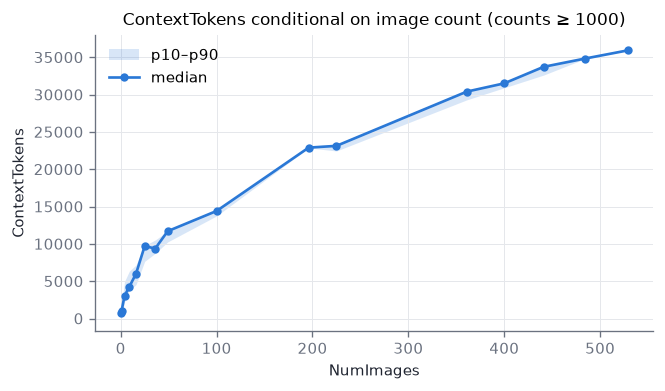
\includegraphics[width=0.72\linewidth]{figuras/eda/eda_a_context_vs_numimages.png}
\caption{Median context tokens conditioned on image count (image-bearing
requests). Context rises monotonically with images but the \emph{per-image}
increment decays --- from ${\approx}277$ tokens at one image to ${\approx}66$
at 529 --- so the vision contribution embedded in \texttt{ContextTokens} is
non-constant and cannot be subtracted out. The converter therefore uses
\texttt{ContextTokens} verbatim as the language-pool input length and drives
encoder work from \texttt{NumImages} separately.}
\label{fig:eda-ctx-vs-img}
\end{figure}

\section{Request anatomy}
\label{sec:eda-requests}

All three request-level marginals are heavy-tailed
(Table~\ref{tab:eda-percentiles}). Generated tokens have a genuinely heavy
tail (Hill index ${\approx}1.9$ on the top percentile), so decode-side
capacity is quantile- rather than mean-driven; context tokens and image
counts have tamer power-law tails (Hill ${\approx}6.6$ and $7.2$). The top
percentile of requests alone carries 15.2\% of all context tokens and 13.4\%
of all generated tokens, so a small fraction of requests dominates both
prefill and decode volume.
Multimodal requests have longer inputs but \emph{shorter} outputs than
text-only requests (context median 1{,}422 vs.\ 792 tokens; generation
median 80 vs.\ 147) --- a question-answering profile against longer-form
text chat.

Unsupervised clustering of all requests on $\log(1{+}\text{images})$,
$\log(1{+}\text{context})$, and $\log(1{+}\text{generated})$ (cuML
$k$-means, $k{=}4$ by silhouette) recovers four interpretable archetypes
(Table~\ref{tab:eda-archetypes}, Figure~\ref{fig:eda-clusters}). The
video/frame-analysis archetype ---
3.4\% of requests --- carries 85.7\% of all image volume and a third of
all prefill tokens, converging with the $k^2$ class structure identified
independently. Each archetype stresses a different serving stage: video
jobs stress the vision encoder and prefill; conversational text stresses
decode; extraction-style requests stress almost nothing.

\begin{table}[htb]
\centering
\caption{Request archetypes recovered by unsupervised clustering.}
\label{tab:eda-archetypes}
\footnotesize
\setlength{\tabcolsep}{4pt}
\begin{tabular}{lrrrl}
\toprule
Archetype & Requests & Image vol. & Prefill vol. & p50 (img/ctx/gen) \\
\midrule
Text: conversational generation & 51.4\% & 1.3\% & 23.9\% & 0 / 1{,}063 / 201 \\
Text: short answer / extraction & 31.0\% & 1.1\% & 9.6\% & 0 / 738 / 22 \\
Vision: document/tiled          & 14.1\% & 11.9\% & 33.5\% & 9 / 4{,}879 / 124 \\
Vision: video/frame analysis    & 3.4\%  & \textbf{85.7\%} & 32.9\% & 400 / 31{,}512 / 56 \\
\bottomrule
\end{tabular}
\end{table}

\begin{figure}[htb]
\centering
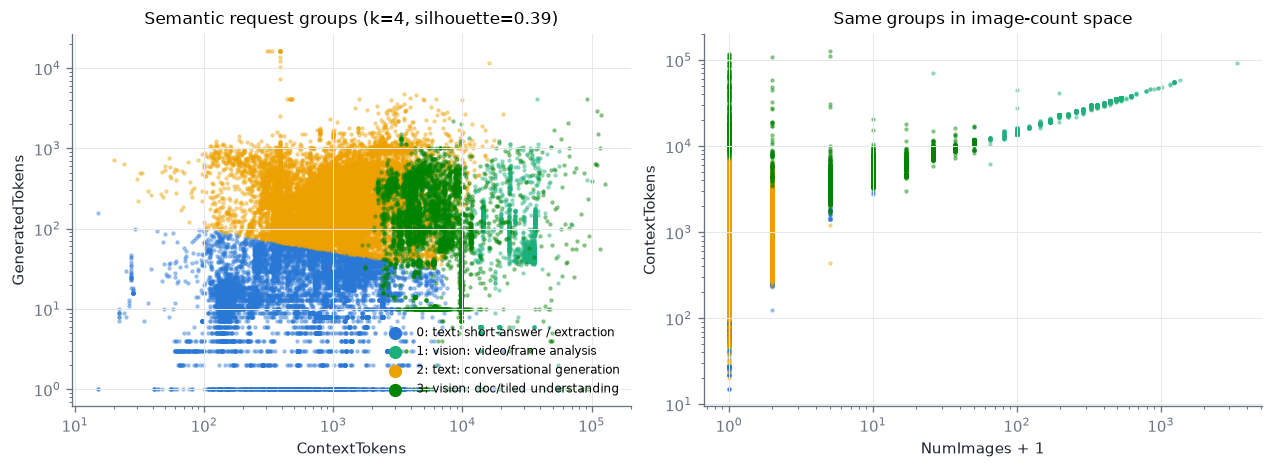
\includegraphics[width=\linewidth]{figuras/eda/eda_l_request_clusters.png}
\caption{Unsupervised $k$-means archetypes ($k{=}4$ by silhouette). Left:
requests in the (context, generation) plane; the two text archetypes (blue,
orange) separate by output length, the two vision archetypes (green) by scale.
Right: the same groups in image-count space, where the video/frame archetype
occupies the high-\texttt{NumImages} tail. A single serving endpoint receives
four workloads that each stress a different stage --- decode, encoder, or
prefill --- which is the disaggregation argument stated at the workload level.}
\label{fig:eda-clusters}
\end{figure}

\section{Temporal structure}
\label{sec:eda-temporal}

The arrival process is not Poisson at any operationally relevant scale:
inter-arrival coefficient of variation 1.55, overdispersed per-second
counts, and a Fano factor that grows without bound with the counting
window --- 1.8 at \SI{1}{\second}, 31.9 at one minute, 938 at one hour
(Figure~\ref{fig:eda-arrival}).
No aggregation window smooths the burstiness away. Spectrally, a real
diurnal harmonic family (\SI{24}{\hour} line with 12/8/\SI{6}{\hour}
overtones; in the request signal the 12- and 8-hour harmonics exceed the
24-hour fundamental, indicating a multi-peaked daily profile) sits on a
strong $1/f^{\beta}$ long-range-dependent background. A bin-exact
significance test rejects any sub-diurnal spectral line, and periods of
\SI{84}{\hour} and above are record-length artifacts of the seven-day
window rather than weekly cycles.

\begin{figure}[htb]
\centering
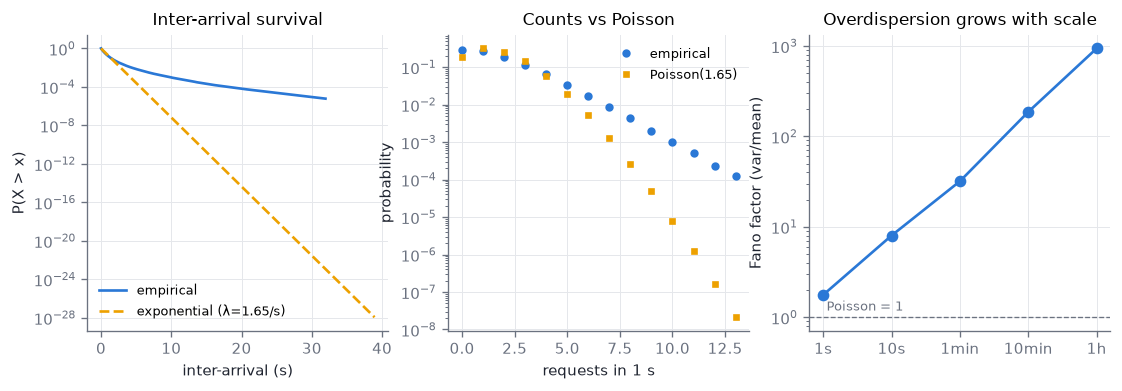
\includegraphics[width=\linewidth]{figuras/eda/eda_e_arrival_process.png}
\caption{The arrival process is not Poisson at any scale. Left: the empirical
inter-arrival survival curve is far heavier than the matched exponential.
Middle: per-second counts are overdispersed against Poisson$(1.65)$. Right: the
Fano factor climbs from $1.8$ at \SI{1}{\second} to $938$ at one hour instead of
staying at the Poisson value of $1$ --- burstiness is scale-free, so no
aggregation window smooths it away and reactive smoothing alone cannot absorb
it.}
\label{fig:eda-arrival}
\end{figure}

\begin{figure}[htb]
\centering
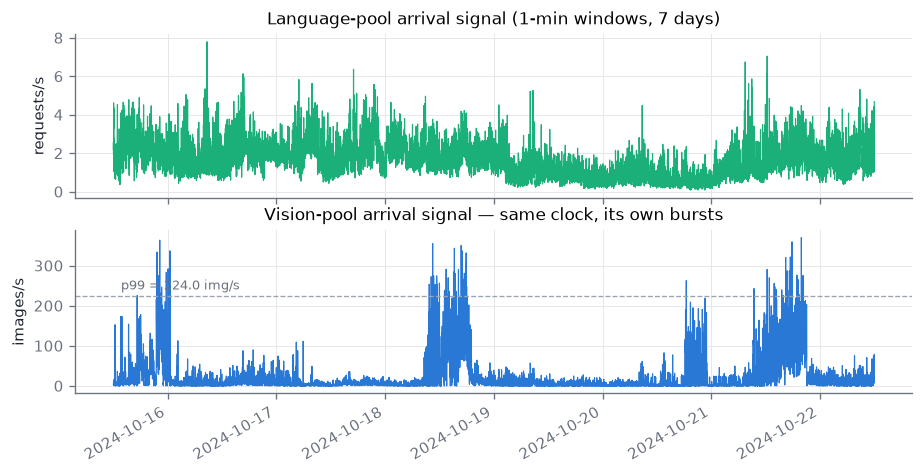
\includegraphics[width=\linewidth]{figuras/eda/eda_c_seven_day_signals.png}
\caption{The two pools' arrival signals over the full week on a shared clock.
The language-pool request rate (top) is quasi-stationary around its mean;
the vision-pool image rate (bottom) is dominated by a handful of multi-hour
burst regimes that pierce the p99 line (dashed) while the request rate barely
moves. The vision signal a rate-based autoscaler never sees is exactly where the
load lives.}
\label{fig:eda-sevenday}
\end{figure}

Table~\ref{tab:eda-persistence} summarizes the four demand signals at
one-minute resolution. Two regularities emerge. The more vision-driven a
signal, the burstier it is; and the more vision-driven, the more
persistent (higher Hurst exponent, longer autocorrelation half-life).
Three independent estimators --- Fano growth, autocorrelation half-life,
and spectral slope --- agree on this ordering. On the same one-minute clock
the vision signal is roughly $12\times$ burstier than the request signal
(CV$^2$ 3.83 vs.\ 0.32) and swings much further above its own mean (peak/mean
$15.6\times$ vs.\ $4.7\times$). One series-construction
caveat applies: all rate signals attribute a request's full token volume
to its arrival minute (the trace carries no durations). This is faithful
for images and prefill, which execute near arrival, but makes the decode
series an \emph{offered-work arrival} signal; actual decode load is a
smoothed, lagged version, so the decode burstiness reported here is an
upper bound.

\begin{table}[htb]
\centering
\caption{Demand signals at 1-minute resolution: burstiness and persistence.}
\label{tab:eda-persistence}
\begin{tabular}{lrrrr}
\toprule
Signal & CV$^2$ & ACF half-life & Spectral slope & Hurst \\
\midrule
requests/s            & 0.32 & \SI{9}{\minute}  & $1/f^{0.66}$ & ${\approx}0.83$ \\
context tokens/s      & 0.85 & \SI{15}{\minute} & $1/f^{0.72}$ & ${\approx}0.86$ \\
\quad vision-borne part & --- & ---             & $1/f^{0.74}$ & ${\approx}0.87$ \\
\quad text-borne part   & --- & ---             & $1/f^{0.51}$ & ${\approx}0.76$ \\
generated tokens/s    & 0.40 & \SI{5}{\minute}  & $1/f^{0.82}$ & ${\approx}0.91$ \\
images/s              & \textbf{3.83} & \textbf{\SI{69}{\minute}} & $1/f^{0.86}$ & $\boldsymbol{{\approx}0.93}$ \\
\bottomrule
\end{tabular}
\end{table}

\section{The vision signal: decoupled, bursty, single-class}
\label{sec:eda-vision}

A constant-fraction model --- vision work as a fixed multiple of request
rate --- explains only $R^2 = \num{0.123}$ of the image-rate series
($\alpha = 15.1$ images per request; Figure~\ref{fig:eda-decouple}), while
decode load is largely carried
by request rate ($R^2 = \num{0.654}$; Pearson $r$ against request rate is
$0.36$ for images versus $0.81$ for decode). The request-rate signal, the input
of conventional autoscalers, contains most of the information about decode
demand and almost none about vision demand. What any scaling policy can do
with this depends on system parameters (cold-start time, per-replica
capacity, cost) outside this dataset; the dataset establishes the
information asymmetry itself.

\begin{figure}[htb]
\centering
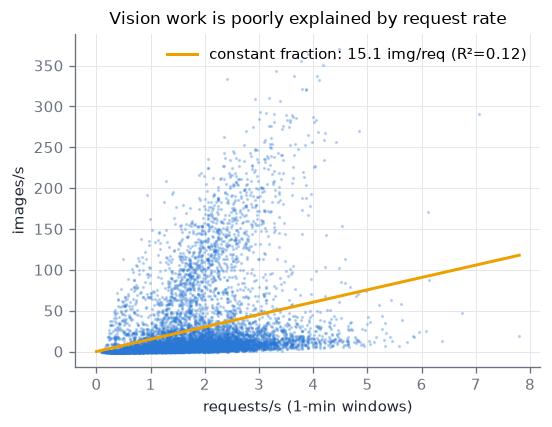
\includegraphics[width=0.72\linewidth]{figuras/eda/eda_d_img_vs_req_scatter.png}
\caption{Image rate against request rate over one-minute windows. The
best-fit constant-fraction line ($15.1$ img/req) explains only $R^2 = 0.12$:
the same request rate coincides with image rates spanning two orders of
magnitude, and the highest image-rate windows are not the highest request-rate
windows. Request rate --- the signal a conventional autoscaler watches ---
carries almost no information about vision load.}
\label{fig:eda-decouple}
\end{figure}

The image-rate signal exceeds its 99th percentile (\num{224}~images/s) in
87 one-minute windows forming 18 contiguous episodes. The largest episode
peaks at \num{370}~images/s while the request rate peaks at only
\num{4.48} requests/s --- bursts are invisible in the request signal
(Figure~\ref{fig:eda-sevenday}).
Episode composition is remarkably homogeneous: the frames class ($k>10$,
video-like jobs; 2.7\% of requests, 81.2\% of all image volume) supplies
93--96\% of the image volume of every top episode, and clustering the 18
episodes on shape and composition features isolates a single mixed-composition
outlier against an otherwise uniform population. This trace contains, in
effect, \emph{one burst type} --- frames-class floods varying in magnitude
and duration.

Bursts compound on the prefill side. Multimodal requests carry 72.5\% of
all prefill tokens, and during burst minutes the mean prefill length is
$2.69\times$ that of calm minutes: more images and longer prefills arrive
together (window-level images--context correlation $r=0.89$). Decode is the
mirror image: during the same image bursts the generated-token rate rises only
$1.78\times$, and per-request generation actually \emph{shortens} (median 84
vs.\ 99 tokens) --- the decode pool is nearly burst-neutral while the vision
and prefill stages are not. Finally,
burst onsets are fast: baseline-to-peak in a median of \SI{6}{\minute}
(10th percentile \SI{2}{\minute}, fastest \SI{1}{\minute}), with a median
steepest single-minute jump of \num{208}~images/s. The onset time is the
budget available to any scaling decision; against replica cold-starts of
tens of seconds to minutes, the fast half of these bursts cannot be
tracked reactively (Figure~\ref{fig:eda-onsets}).

\begin{figure}[htb]
\centering
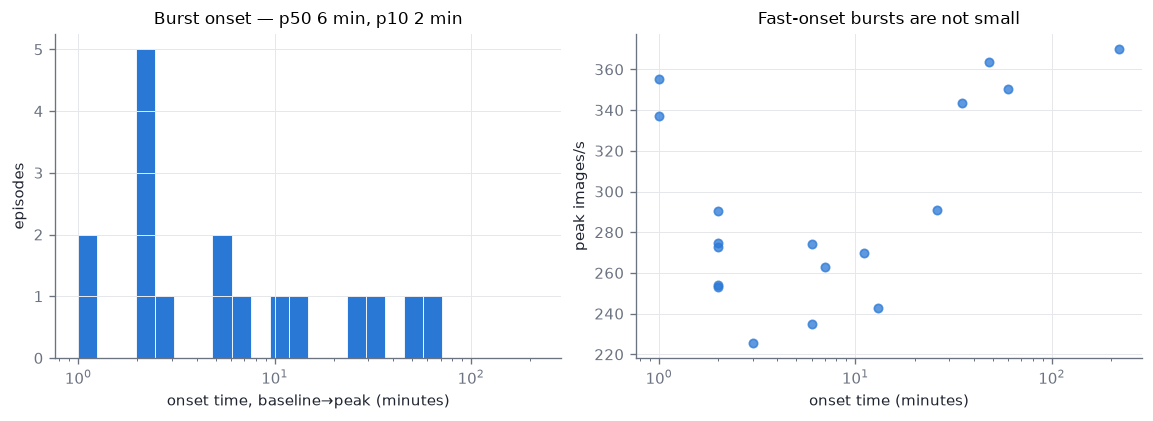
\includegraphics[width=\linewidth]{figuras/eda/eda_i_burst_onsets.png}
\caption{Burst onset speed across the 18 episodes. Left: the baseline-to-peak
ramp time is a median of \SI{6}{\minute}, with the fastest episodes reaching
peak in one to two minutes. Right: fast onset does not mean small
burst --- some of the steepest ramps reach the highest peaks. The onset time is
the entire budget a scaling policy has; the fast half of these episodes ramps
faster than a replica can cold-start, which is what makes reactive scaling
insufficient and forecasting necessary.}
\label{fig:eda-onsets}
\end{figure}

\section{Signal predictability}
\label{sec:eda-predictability}

The image signal pairs the highest burstiness with the strongest
persistence: 69 minutes of autocorrelation half-life
(autocorrelation 0.64 at a 5-minute lag) and $H \approx 0.93$
(Figure~\ref{fig:eda-acf}). The signal
most dangerous to reactive scaling is precisely the one with the most
forecastable structure at provisioning horizons. Its long-range dependence
also implies that short-memory models (Poisson or low-order ARMA) will
structurally underfit it.

\begin{figure}[htb]
\centering
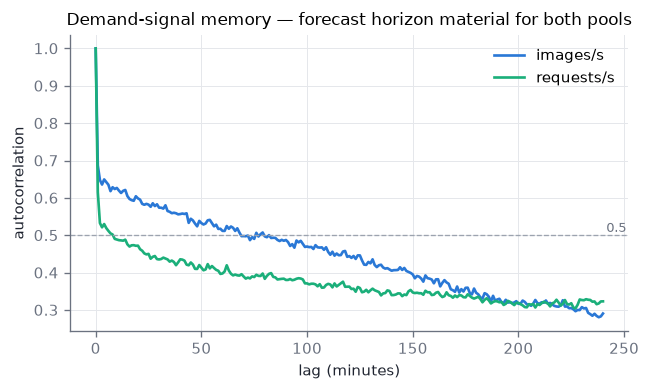
\includegraphics[width=0.72\linewidth]{figuras/eda/eda_d_acf.png}
\caption{Autocorrelation of the two arrival signals versus lag. The image
signal (blue) retains autocorrelation $0.64$ at a five-minute lag and crosses
$0.5$ only at \SI{69}{\minute}, against \SI{9}{\minute} for the request signal
(green). The demand most invisible to request-rate monitoring is also the most
forecastable at exactly the horizons provisioning needs --- the feasibility
premise for the predictive-scaling contribution.}
\label{fig:eda-acf}
\end{figure}

The demand signals are not derivable from one another. At request level,
image count and generation length are independent (Spearman $-0.06$;
median generation stays at 50--140 tokens across image counts from 1 to
529). At window level, the image--generation cross-correlation peaks
sharply at lag zero with no lead. Neither request rate nor any pool's
signal proxies another's: each of the three demand signals (images/s,
context tokens/s, generated tokens/s) carries information the others do
not. Below the one-minute scale, all signals reach a white shot-noise
floor: finer-grained inputs add noise, not information --- though the
decision frequency a serving system actually requires depends on
cold-start, capacity, and cost parameters that this dataset does not
contain.

\section{Resolution sensitivity and tail regimes}
\label{sec:eda-multires}

The burstiness results depend on the observation window, and the dependence is
not the same for every signal. Table~\ref{tab:eda-multires} tracks, for each
signal, the peak observed at a given window size as a fraction of the peak
observed at \SI{1}{\second}. Coarsening the window hides the vision peaks far
faster than the request peaks: at \SI{60}{\second} a monitor still sees 37\% of
the true one-second request peak but only \textbf{3.9\%} of the one-second image
peak (11.2\% for context, 6.5\% for generation). A minute-resolution monitor
therefore understates the encoder pool's instantaneous surges by roughly
$25\times$, while understating the request rate by under $3\times$. The image
signal's excess-dispersion also decays most slowly with window size
(CV$^2$ $25.7\!\rightarrow\!3.83$ from \SI{1}{\second} to \SI{60}{\second};
Figure~\ref{fig:eda-multires}),
consistent with its long-range dependence: no practical aggregation window
recovers a well-behaved image signal.

\begin{table}[htb]
\centering
\caption{Observed peak at each window size as a fraction of the
\SI{1}{\second} peak. Vision peaks vanish under aggregation an order of
magnitude faster than request peaks.}
\label{tab:eda-multires}
\begin{tabular}{lrrrrr}
\toprule
Signal & \SI{1}{\second} & \SI{5}{\second} & \SI{15}{\second} & \SI{60}{\second} & \SI{300}{\second} \\
\midrule
requests/s      & 100\% & 58.1\% & 46.7\% & 37.1\% & 23.4\% \\
context tokens/s & 100\% & 26.8\% & 18.0\% & 11.2\% & 7.4\% \\
generated tokens/s & 100\% & 21.8\% & 12.3\% & 6.5\% & 4.3\% \\
images/s        & 100\% & 20.1\% & 6.9\% & \textbf{3.9\%} & 2.6\% \\
\bottomrule
\end{tabular}
\end{table}

\begin{figure}[htb]
\centering
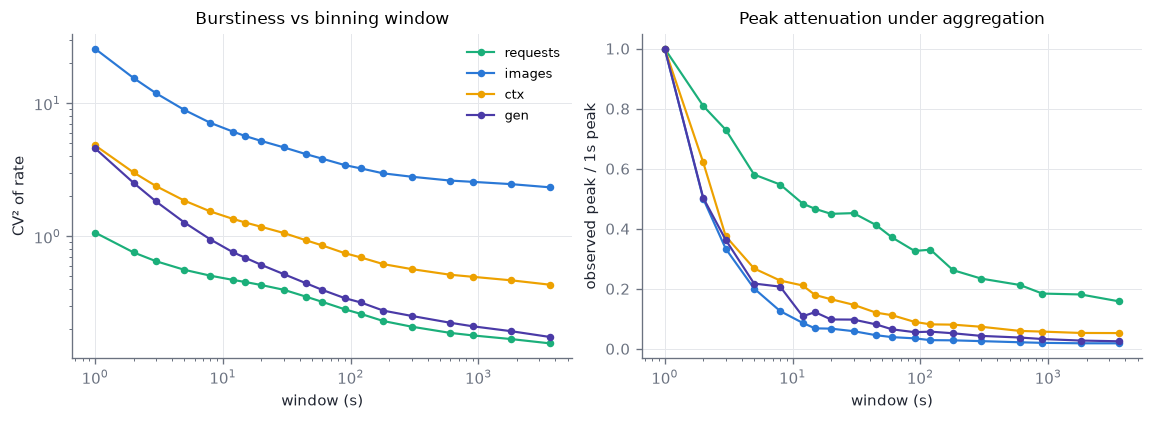
\includegraphics[width=\linewidth]{figuras/eda/eda_q_multires.png}
\caption{Sensitivity to the observation window. Left: excess dispersion
(CV$^2$) versus window size --- the image signal (blue) stays an order of
magnitude burstier than the request signal (green) across every window and
decays the slowest. Right: peak observed at each window as a fraction of the
\SI{1}{\second} peak --- image peaks collapse to ${\approx}4\%$ by
\SI{60}{\second} while request peaks retain ${\approx}37\%$. A coarse monitor
does not merely blur the vision surges, it erases them.}
\label{fig:eda-multires}
\end{figure}

Conditioning the request marginals on their own extremes exposes who occupies
each tail. The top-1\% context-token requests are 81.6\% multimodal with a
median of 529 images --- the large-context tail \emph{is} the frames class, not
long text prompts. The top-1\% image-count requests are 100\% multimodal, carry
a median of ${\approx}\num{36000}$ context tokens (tail-deterministic
image--context coupling), and decode only briefly (median 53 generated tokens).
By contrast the busiest 1\% of request-rate minutes carry ordinary-composition
traffic: median 1 image and median context and generation within a few percent
of the global medians --- high request rate does not imply heavy per-request
work. Most sharply, the minutes of highest request rate and the minutes of
highest image rate barely overlap: of 106 hot-request and 101 hot-image minutes
only \textbf{5} are shared (Jaccard 0.02). The two pools' extreme-load events
are essentially disjoint in time, which is the decoupling result of
Section~\ref{sec:eda-vision} restated at its strongest --- provisioning the
vision pool from the request signal misses precisely the moments that matter.

\section{Global reference percentiles}
\label{sec:eda-globals}

\begin{table}[htb]
\centering
\caption{Global percentiles: request-level marginals and 1-minute rates.}
\label{tab:eda-percentiles}
\footnotesize
\setlength{\tabcolsep}{4pt}
\begin{tabular}{lrrrrrrr}
\toprule
Signal & mean & p50 & p90 & p95 & p99 & p99.9 & max \\
\midrule
NumImages (image-bearing) & 28.7 & 1 & 25 & 196 & 529 & 1{,}089 & 9{,}409 \\
ContextTokens  & 2{,}911 & 1{,}124 & 5{,}828 & 9{,}755 & 35{,}932 & 65{,}623 & 148{,}569 \\
GeneratedTokens & 187 & 98 & 433 & 603 & 1{,}066 & 3{,}943 & 16{,}384 \\
\midrule
requests/s (1-min) & 1.7 & 1.55 & 2.88 & 3.33 & 4.35 & 5.73 & 7.8 \\
images/s (1-min) & 23.7 & 5.6 & 77 & 132 & 224 & 322 & 370 \\
ctx tokens/s (1-min) & 4{,}813 & 3{,}537 & 10{,}326 & 14{,}157 & 21{,}610 & 30{,}647 & 39{,}108 \\
gen tokens/s (1-min) & 309 & 281 & 531 & 629 & 1{,}010 & 1{,}599 & 2{,}164 \\
\bottomrule
\end{tabular}
\end{table}

\section{Limitations}
\label{sec:eda-limitations}

The trace carries no image resolutions (counts only), no session or user
identifiers, and no latency or completion-time ground truth (it is
arrival-side only). Its seven-day window supports diurnal but not weekly
periodicity claims. The 50/50 modality split is by construction. The
context-token field embeds the \emph{traced} model's vision tokenization,
so token counts are self-consistent as a workload but not transferable to
a different model's tokenizer.

\section{Summary}

The trace reveals a workload in which half the requests are text-only,
images arrive as tile/frame batches, and four request archetypes stress
different serving stages. Its arrival process is non-Poisson at every
scale, with diurnal harmonics over a long-range-dependent background. The
vision demand signal is simultaneously the least visible to request-rate
monitoring ($R^2 = 0.123$), the burstiest (CV$^2$ 3.83; single-class
frames floods ramping in a median of six minutes), and the most persistent
($H \approx 0.93$, 69-minute memory) --- while decode demand is largely
rate-carried and comparatively benign. The two are disjoint even at their
extremes: the busiest request-rate minutes and the busiest image-rate minutes
scarcely coincide (5 shared of ${\approx}100$ each), and minute-resolution
monitoring recovers under 4\% of the true instantaneous image peak. These are
properties of the
dataset; their consequences for serving-system design are developed in the
chapters that follow.


% Minimal bibliography so the build resolves \cite without biber.
\begin{thebibliography}{9}
\bibitem{Qiu2025ModServe}
S.~Qiu, X.~Liu, et al.
\emph{ModServe: Modality-Disaggregated Serving for Multimodal LLM Inference}.
ACM SoCC, 2025. arXiv:2502.00937.
\end{thebibliography}

\end{document}
